% !TEX program  = pdflatex
\documentclass{article}
\usepackage[ruled,vlined,linesnumbered]{algorithm2e}
\usepackage{algpseudocode}
\usepackage{amsmath}
\usepackage{amsthm}
\usepackage{graphicx}
\usepackage{subfigure}
\usepackage{float}
\usepackage{amsmath }
\usepackage{amsfonts }
\usepackage{pdfpages}
\usepackage{epsfig}
\usepackage{graphicx}
\usepackage{arydshln}
\usepackage{verbatim}
\usepackage{subfigure}
\usepackage{enumerate}
\usepackage{rotating}
\usepackage{threeparttable}
\usepackage{caption}
\usepackage{epsfig}
\usepackage{cite}
\usepackage{geometry}
\geometry{a4paper, top=2.54cm, bottom=2.54cm, left=3.18cm, right=3.18cm}
\theoremstyle{definition}
\newtheorem{prob}{Problem}
\newtheorem{ans}{Answer}
\usepackage[colorlinks,linkcolor=black]{hyperref}
\linespread{1.2}
\begin{document}
	\title{CS257 Linear and Convex Optimization Homework 6 }
	\author{Kailing Wang 521030910356}
	\date{November 15.2022}
	\maketitle
	For this assignment, you should submit a pdf file as well as your source code (.py files). The pdf file should include all necessary figures, the outputs of your Python code, and your answers to the questions. Do NOT write your answers in any of the .py files.
	
	In this assignment, you will implement gradient descent with constant step size. First complete the function gd\_const\_ss in gd.py.
	
	\begin{prob}
	Consider the following quadratic program,

	
	$$
	\min _{\boldsymbol{x} \in \mathbb{R}^{2}} f(\boldsymbol{x})=\frac{1}{2} \boldsymbol{x}^{T} \boldsymbol{Q} \boldsymbol{x}
	$$
	
	where
	
	$$
	\boldsymbol{Q}=\left(\begin{array}{ll}
		1 & 0 \\
		0 & \gamma
	\end{array}\right)
	$$
	
	with $\gamma>0$. In terms of coordinates,
	
	$$
	f\left(x_{1}, x_{2}\right)=\frac{1}{2} x_{1}^{2}+\frac{\gamma}{2} x_{2}^{2} .
	$$
	
	We know the optimal solution is $\boldsymbol{x}^{*}=\mathbf{0}$ and $f^{*}=f\left(\boldsymbol{x}^{*}\right)=0$.
	
	(a). What is the smallest $L$ such that $f$ is $L$-smooth?
	
	(b). Suppose $\gamma=10$. Complete p1.py and run the gradient descent algorithm you implemented with step sizes $0.22,0.1,0.01,0.001$. (Note: for step size $0.22$, you may want to limit the maximum number of iterations to a small number, say 10.) Does it converge in each case? When it does converge, how many iterations does it take? In each case, plot the $2 \mathrm{D}$ trajectory of the sequence $\boldsymbol{x}_{k}$ and the function values $f\left(\boldsymbol{x}_{k}\right)$. You can use the function provided in utils.py or write your own code. Note that $f\left(\boldsymbol{x}_{k}\right)$ is also the approximation error since $f\left(\boldsymbol{x}^{*}\right)=0$.
	
	(c). For $\gamma=1,0.1,0.01,0.001$, run gradient descent with step size 1 . How many iterations do you need in each case? How does the number of iterations change as $\gamma$ decreases?
	\end{prob}

	\begin{ans}
		\begin{enumerate}[(a)]
			\item $$||\nabla f(x)-\nabla f(y)||=||x_1+\gamma\cdot x_2-y_1-\gamma\cdot y_2||
			$$
			That is, if $\gamma>1$, we have $$||\nabla f(x)-\nabla f(y)||\leq \gamma\cdot||\boldsymbol{x}-\boldsymbol{y}||$$
			f is $\gamma-$smooth. 
			
			If $0<\gamma\leq1$, we have $$||\nabla f(x)-\nabla f(y)||\leq ||\boldsymbol{x}-\boldsymbol{y}||$$
			f is $1-$smooth. 
			\item The case for step size 0.22 did not converge. In all other cases, it converges. 
			
			Step size 0.1 case converges after 11 iterations. Step size 0.01 case converges after 1147 iterations, and step size 0.001 case converges after 11509 iterations. The graph is attached in the document.
			
			\begin{figure}
				\begin{minipage}[t]{0.48\textwidth}
					\centering
					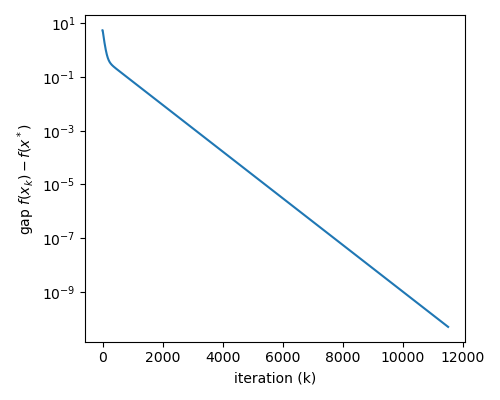
\includegraphics[width=0.7\linewidth]{../figures/gd_f_gamma10_ss0.001}
					\caption{gd\_f\_gamma10\_ss0.001}
				\end{minipage}
				\begin{minipage}[t]{0.48\textwidth}
					\centering
					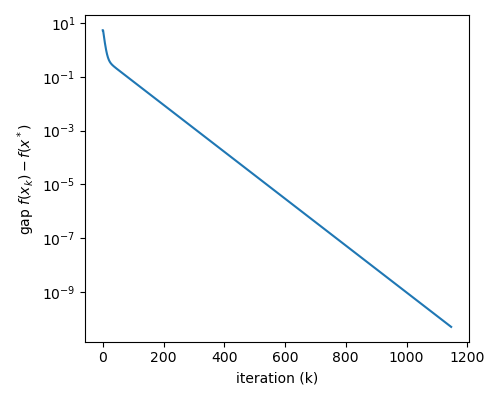
\includegraphics[width=0.7\linewidth]{../figures/gd_f_gamma10_ss0.01}
					\caption{gd\_f\_gamma10\_ss0.01}
				\end{minipage}
				\begin{minipage}[t]{0.48\textwidth}
					\centering
					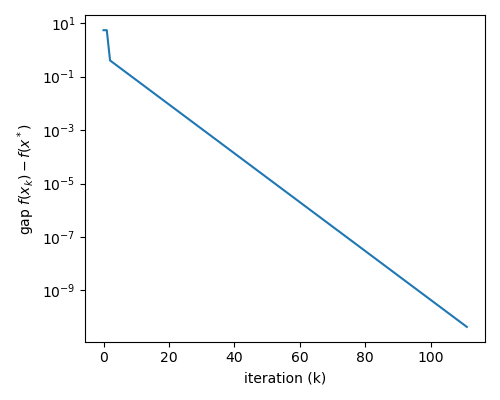
\includegraphics[width=0.7\linewidth]{../figures/gd_f_gamma10_ss0.1}
					\caption{gd\_f\_gamma10\_ss0.1}
				\end{minipage}
				\begin{minipage}[t]{0.48\textwidth}
					\centering
					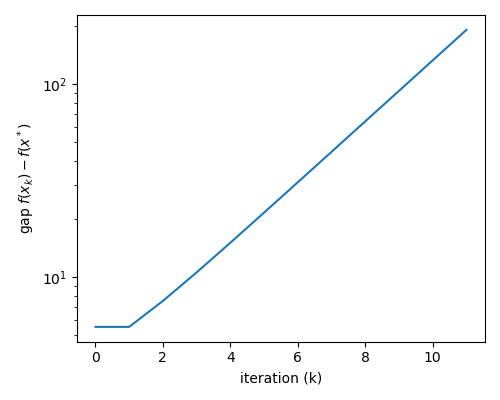
\includegraphics[width=0.7\linewidth]{../figures/gd_f_gamma10_ss0.22}
					\caption{gd\_f\_gamma10\_ss0.22}
				\end{minipage}
			\end{figure}
			\begin{figure}
				\begin{minipage}[t]{0.48\textwidth}
					\centering
					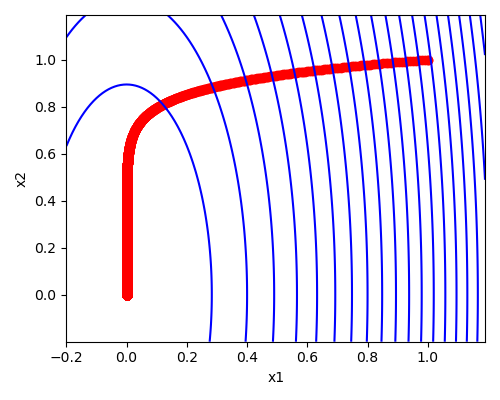
\includegraphics[width=0.7\linewidth]{../figures/gd_traces_gamma10_ss0.001}
					\caption{gd\_traces\_gamma10\_ss0.001}
				\end{minipage}
				\begin{minipage}[t]{0.48\textwidth}
					\centering
					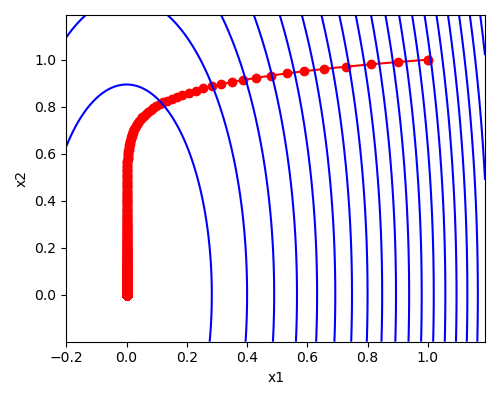
\includegraphics[width=0.7\linewidth]{../figures/gd_traces_gamma10_ss0.01}
					\caption{gd\_traces\_gamma10\_ss0.01}
				\end{minipage}
				\begin{minipage}[t]{0.48\textwidth}
					\centering
					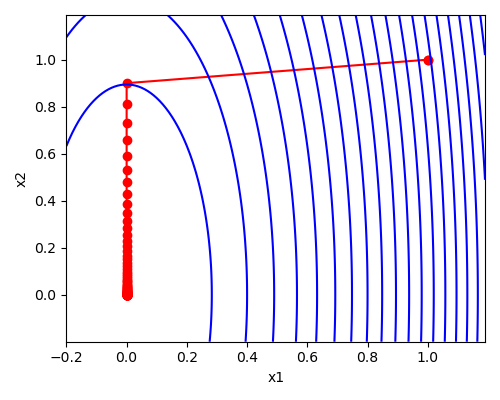
\includegraphics[width=0.7\linewidth]{../figures/gd_traces_gamma10_ss0.1}
					\caption{gd\_traces\_gamma10\_ss0.1}
				\end{minipage}
				\begin{minipage}[t]{0.48\textwidth}
					\centering
					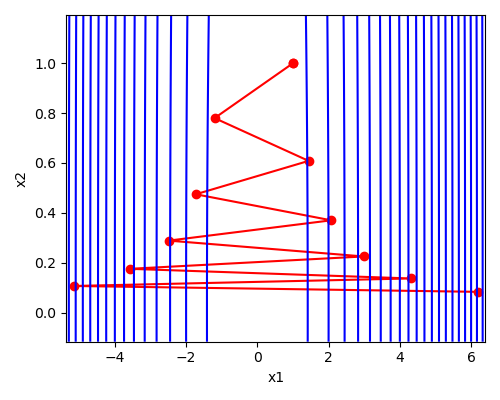
\includegraphics[width=0.7\linewidth]{../figures/gd_traces_gamma10_ss0.22}
					\caption{gd\_traces\_gamma10\_ss0.22}
				\end{minipage}
			\end{figure}
			\item For $\gamma = $ 1, 0.1, 0.01, 0.001, the gradient descent needs 2, 89, 689, 4604 iterations. The iteration needed grows as $\gamma$ decreases. 
		\end{enumerate}
	\end{ans}

	\begin{prob}
	Consider the least squares problem in Problem 3(a) of Homework 5, i.e.

	$$
	\min _{\boldsymbol{w}}\|\boldsymbol{X} \boldsymbol{w}-\boldsymbol{y}\|_{2}^{2}
	$$
	
	where
	
	$$
	\boldsymbol{X}=\left(\begin{array}{cccccc}
		4 & 1 & 0 & 4 & 2 & 0 \\
		2 & 4 & 1 & 1 & 0 & 2 \\
		4 & 4 & 0 & 4 & 1 & 4 \\
		1 & 0 & 2 & 3 & 1 & 2 \\
		4 & 4 & 2 & 2 & 0 & 1 \\
		2 & 2 & 0 & 1 & 2 & 4 \\
		0 & 1 & 2 & 1 & 4 & 2 \\
		0 & 0 & 1 & 0 & 1 & 3
	\end{array}\right), \quad \boldsymbol{y}=\left(\begin{array}{l}
		5 \\
		0 \\
		5 \\
		0 \\
		4 \\
		2 \\
		5 \\
		3
	\end{array}\right)
	$$
	
	Use your implementation of gradient descent to solve this least squares problem. You may follow provided codes of problem 1. Use any stepsize you find appropriate. Compare your solution with the solution you found in HW5, and the solution you find by solving the normal equation using np.linalg.solve.
	\end{prob}

	\begin{ans}
		Set initial point $\boldsymbol{0}$ and step size 0.001, the gradient descent converges after 4180 iterations and output 
		$$
		[[ 1.22170436]
		[-0.21469164]
		[ 0.1554913 ]
		[-0.45867604]
		[ 1.18537713]
		[ 0.00613276]]
		$$ as result. Plot p2\_ss0.001 shows the process.
		
		\begin{figure}
			\centering
			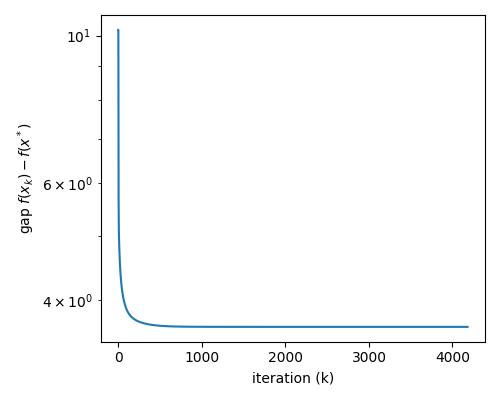
\includegraphics[width=0.5\linewidth]{../figures/p2_ss0.001}
			\caption{p2\_ss0.001}
			\label{fig:p2ss0}
		\end{figure}		
		
		In hw5 I used np.linalg.solve to solve function $\nabla (\|\boldsymbol{X} \boldsymbol{w}-\boldsymbol{y}\|_{2}^{2})=2\cdot\boldsymbol{X^T}\cdot(\boldsymbol{X} \boldsymbol{w}-\boldsymbol{y})=0$, and the result is 
		$$
		[[ 1.22170662]
		[-0.21469307]
		[ 0.15549204]
		[-0.4586777 ]
		[ 1.18537706]
		[ 0.00613317]]
		$$ 
		
		They are very much the same.
	\end{ans}

	\begin{prob}
	Logistic regression. In this problem, you will train a logistic regression classifier on a toy dataset given in p3.py. The features are two dimensional, so the $i$-th sample is $\left(\boldsymbol{x}_{i}, y_{i}\right) \in \mathbb{R}^{2} \times\{+1,-1\}$. As in Problem 2 of Homework 1, we will append a constant 1 to each $\boldsymbol{x}_{i}$ to make it three dimensional, and absorb the bias term $b$ into $\boldsymbol{w}$ by defining a new $\boldsymbol{w}=\left(w_{1}, w_{2}, b\right)^{T} \in \mathbb{R}^{3}$. The objective function to be minimized is
	
	$$
	f(\boldsymbol{w})=\sum_{i=1}^{m} \log \left(1+e^{-y_{i} \boldsymbol{x}_{i}^{T} \boldsymbol{w}}\right)
	$$
	
	where $m$ is the number of samples. Its gradient is found in Problem 2(c) of HW1,
	
	$$
	\nabla f(\boldsymbol{w})=-\sum_{i=1}^{m}\left[1-\sigma\left(y_{i} \boldsymbol{x}_{i}^{T} \boldsymbol{w}\right)\right] y_{i} \boldsymbol{x}_{i}
	$$
	
	where $\sigma(z)=1 /\left(1+e^{-z}\right)$ is the sigmoid function.
	
	Find the optimal $\boldsymbol{w}^{*}$ using your implementation of gradient descent in gd.py. Report the classification accuracy of the classifier on the training dataset given by
	
	$$
	\text { accuracy }=\frac{1}{m} \sum_{i=1}^{m} \mathbb{1}\left\{y_{i}=\hat{y}_{i}\right\}
	$$
	
	where $\hat{y}_{i}=\operatorname{sgn}\left(\left\langle\boldsymbol{w}^{*}, \boldsymbol{x}_{i}\right\rangle\right)$. You can follow the guidance of p3.py or write your own code. Use matrix operations to calculate the function values and gradients. You may need some of the following functions, numpy.matmul, numpy.multiply, numpy.exp, numpy.reshape.
	\end{prob}

	\begin{ans}
		\begin{figure}
			\centering
			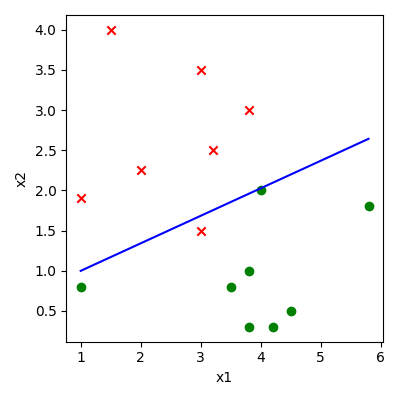
\includegraphics[width=0.5\linewidth]{../figures/p3}
			\caption{Problem 3 curve}
			\label{fig:p3}
		\end{figure}
	
		Converged after 21421 iterations. The dataset is not linear separable. The result of the logic regression is the best linear solution. 
	\end{ans}
\end{document}